\documentclass{article}
    \usepackage{amssymb}
    \usepackage[utf8]{inputenc}
    \usepackage[russian]{babel}
    \usepackage[left=2cm,right=2cm,
        top=2cm,bottom=2cm,bindingoffset=0cm]{geometry}
    \usepackage{hyperref}
    \hypersetup{
        colorlinks=true,
        linkcolor=blue,
        filecolor=magenta,      
        urlcolor=cyan,
    }
  \usepackage{graphicx}
  \graphicspath{{pictures/}}
  \DeclareGraphicsExtensions{.pdf,.png,.jpg}

\begin{document}
\begin{center}{\hugeОтчет по курсовой работе за неделю\\}\end{center}
Дата: 8.10.2020\\
Научные руководители: Герасимов С.В., Мещеряков А.В.\\
Студент: Немешаева Алиса\\
Курс: 4\\

\renewcommand{\labelitemi}{$\blacksquare$}
\renewcommand\labelitemii{$\square$}
\begin{enumerate}
    \item На этой неделе проводилось исследование различных нейросетевых архитектур, которые могут
        улучшить результаты существующих моделей. Были изучены следующие модели:\\
        \begin{itemize}
            \item \hyperlink{https://arxiv.org/pdf/1612.01105.pdf}{PSPNet}\\ 
            \item \hyperlink{https://arxiv.org/pdf/1707.03718.pdf}{LinkNet}\\
            \item \hyperlink{https://arxiv.org/pdf/2009.01907.pdf}{W-Net}\\
        \end{itemize}
    \item На базе обученной ранее модели были созданы каталоги с детектированными скоплениями 
        галактик.\\

\end{enumerate}

\begin{figure}[h]
    \begin{minipage}[h]{0.47\linewidth}
        \center{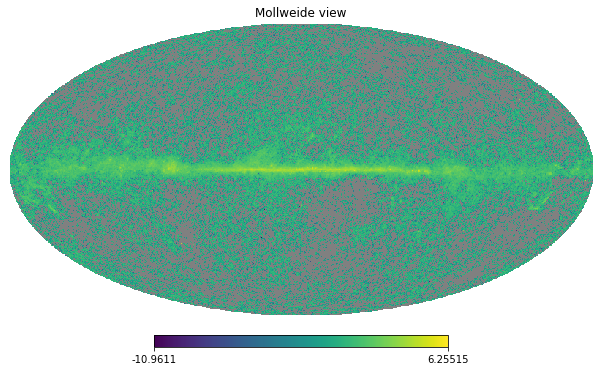
\includegraphics[width=1\linewidth]{100}} 100 \\
    \end{minipage}
\hfill
    \begin{minipage}[h]{0.47\linewidth}
        \center{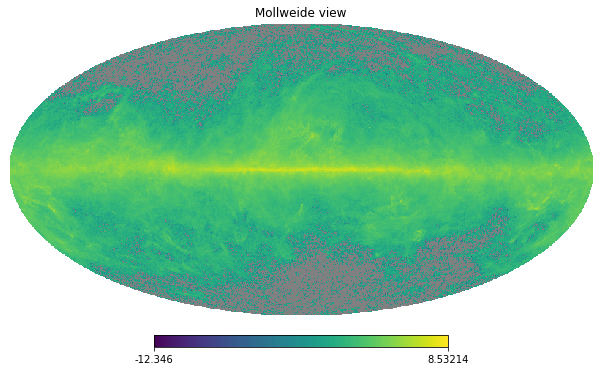
\includegraphics[width=1\linewidth]{353}} \\353
    \end{minipage}
\vfill
    \begin{minipage}[h]{0.47\linewidth}
        \center{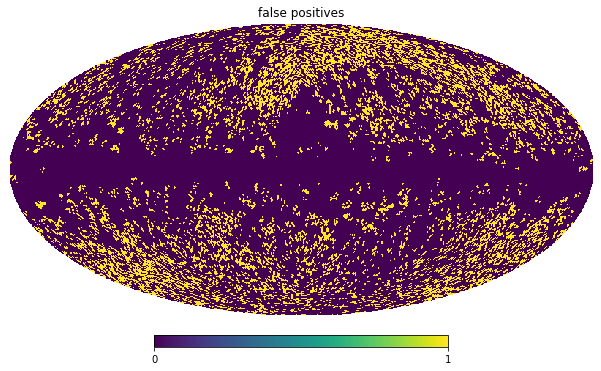
\includegraphics[width=1\linewidth]{fp}} false positives \\
    \end{minipage}
\hfill
    \begin{minipage}[h]{0.47\linewidth}
        \center{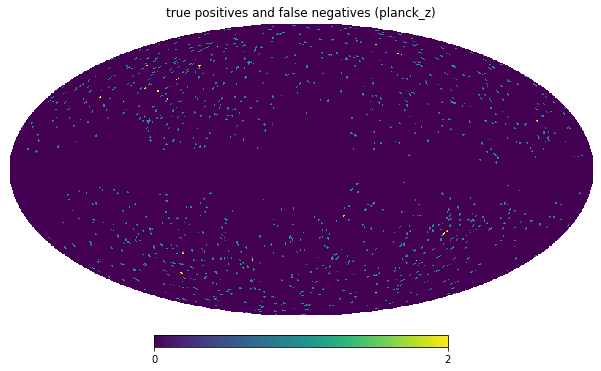
\includegraphics[width=1\linewidth]{planck_z}} planck\_z \\
    \end{minipage}
    \caption{Сигнал микроволновых данных Planck по двум каналам 100 и 353. (Данные, на которых
        проводилась детекция) и карта каталога с результатами сканирования всего неба для модели 
        на 14 эпох с порогом 0.4 для маски сегментации: false positives (объекты, не найденные в 
        выбранных каталогах) и true positives / false negatives для каталога planck\_z, на данных 
        которого обучалась модель}
\end{figure}
На изображении каталога planck\_z синие точки соответствуют true positives, жёлтые - false 
negatives. Общий recall для этой конфигурации для этого каталога составил 0.785 (по всей области 
неба).\\
\textbf{Общее количество строк кода за эту неделю: 63}\\

\newpage

\begin{center}{\huge Сравнение нескольких нейросетевых архитектур\\}\end{center}
\section{PSPNet}
Эта модель была создана для использования в области scene parsing. Главная задача, которую эта 
модель помогает решить - попиксельная сегментация объектов на изображении при условии наличия 
большого количества меток (например, датасет ADE20K, о котором идёт речь в статье, содержит 
изображения с 150 метками). \\

PSPNet помогает решить проблемы:\\
\begin{itemize}
    \item взаимосвязи меток (например, объект 
        с меткой <<самолёт>> скорее всего будет находиться в пространстве с меткой <<аэропорт>> или 
        <<посадочная полоса>>)\\
    \item совпадающих категорий (наличие в тренировочной выборке объектов вроде <<поле>> и <<земля>>, 
        <<холм>> и <<гора>>)\\
    \item небольших объектов (например, <<фонарь>> или <<вывеска>>, находящиеся на дальнем плане 
        изображения)\\
\end{itemize}

Из вышеперечисленных проблем в текущей работе по сегментации скоплений нас может интересовать только 
последняя - искомое скопление может занимать маленькую площадь относительно всего изображения.\\

Основная идея PSPNet заключается в использовании Pyramid Pooling Module. Чтобы получить этот модуль, 
нужно сначала сделать несколько версий изначального изображения в разных масштабах с помощью pooling 
слоёв разных размеров, первый <<грубый>> слой собирает данные всего изображения в один многоканальный 
пиксель, следующий содержит данные нескольких подрегионов, и далее каждый последующий содержат всё 
меньше глобальной информации и всё больше локальной. \\

Далее для каждого масштаба проводится свёртка для уменьшения количества каналов и upscaling с помощью 
билинейной интерполяции, и все масштабы конкатенируются, чтобы с помощью последнего слоя свёртки 
получить для них итоговую сегментацию. \\

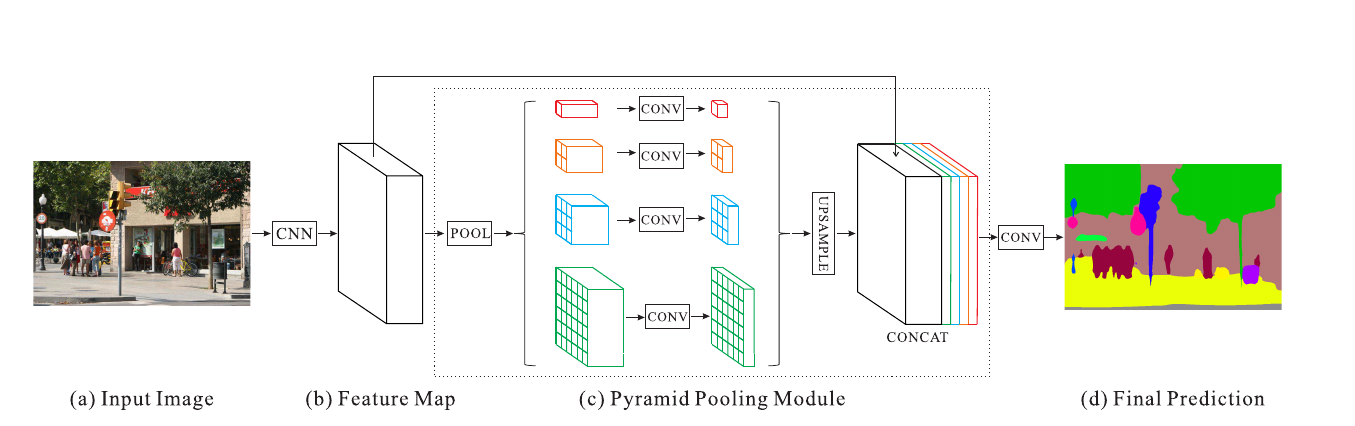
\includegraphics[width=\linewidth]{ppm}

\section{LinkNet}
Эта модель решает проблему большого количества параметров и низкой скорости других моделей из 
похожей области применения. LinkNet хорошо подойдёт для сегментации в реальном времени и сегментации 
на видео, что тоже имеет очень слабое отношение к нашей области, где количество данных фиксировано и 
сегментация в реальном времени не требуется, однако скорость нейросетевой модели тем не менее является 
плюсом.\\

Общая структура LinkNet очень напоминает UNet, с тем отличием, что в блоках кодировщика добавлены 
дополнительные skip-connection связи.\\


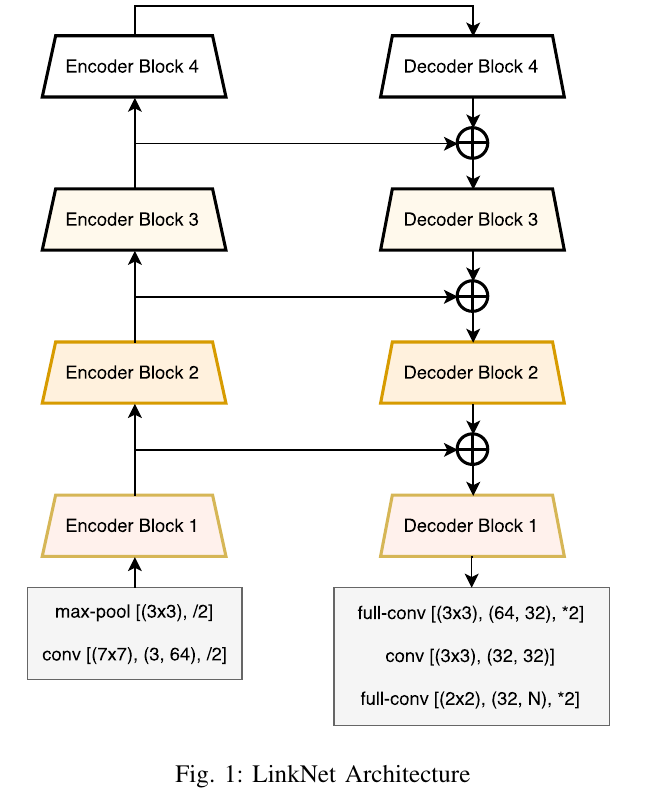
\includegraphics[width=0.3\linewidth]{linknet}
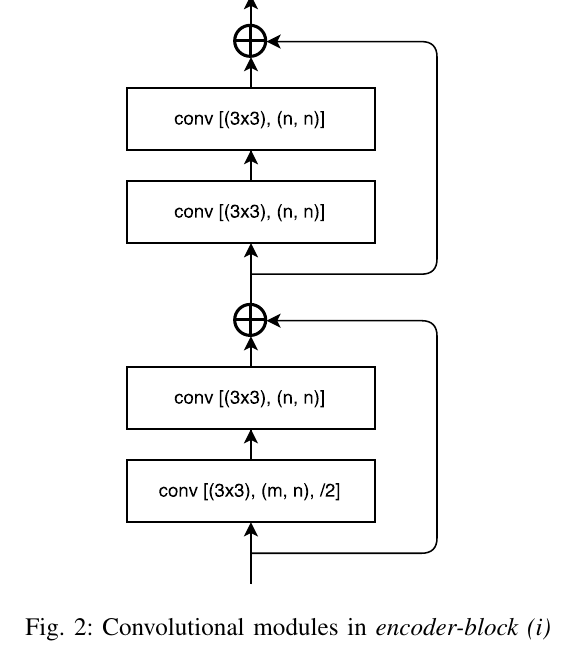
\includegraphics[width=0.3\linewidth]{link_encoder}
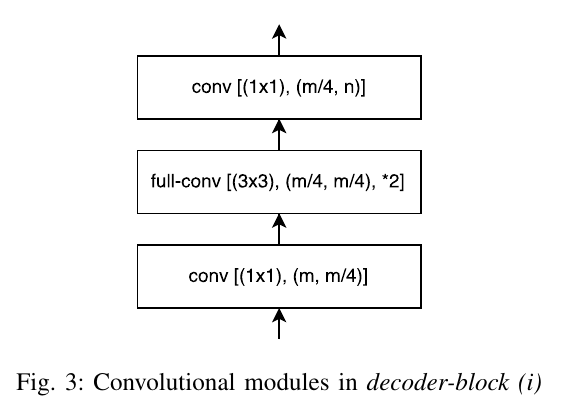
\includegraphics[width=0.3\linewidth]{link_decoder}\\

\section{W-Net}
Эта архитектура была призвана улучшить результаты сегментации при условиях:\\

\begin{itemize}
    \item без использования сложных архитектур свёрточных нейронных сетей\\ 
    \item при тестировании на данных из разных датасетов\\
\end{itemize}

При сегментации космических данных мы обычно имеем общий обзор некоторой области неба в 
определенном спектре, и эти данные получены с помощью определенного телескопа. Однако возможно 
появится причина обучать модель на данных одного телескопа, а тестировать на других, что в какой-то 
степени кореллирует с описанными условиями.\\

Архитектура W-Net предлагает улучшение модели U-Net: обучение происходит на двух последовательных 
нейросетевых моделях. Выход первой модели конкатенируется с входом и отправляется на обработку второй 
моделью.\\

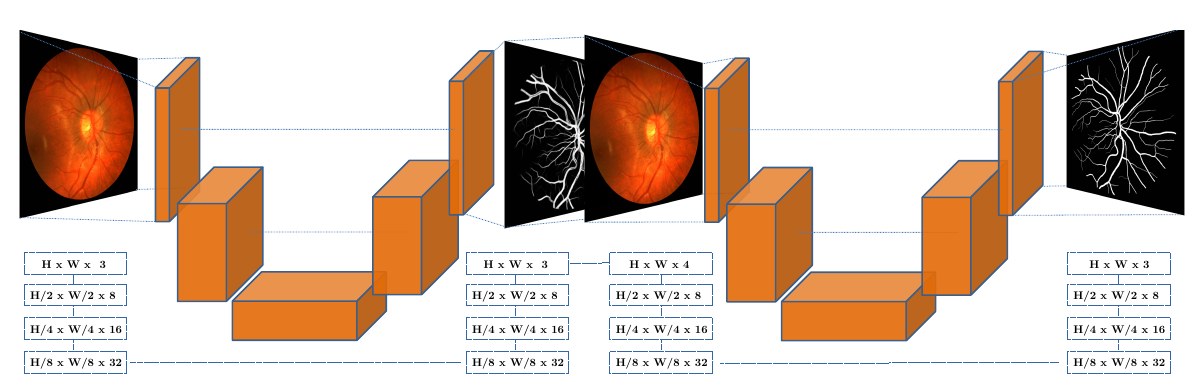
\includegraphics[width=\linewidth]{wnet}\\

\end{document}
